
% Many thanks to Andrew West for writing most of this file
% Main LaTeX file for CIS400/401 Project Proposal Specification
%
% Once built and in PDF form this document outlines the format of a
% project proposal. However, in raw (.tex) form, we also try to
% comment on some basic LaTeX technique. This is not intended to be a
% LaTeX tutorial, instead just (1) a use-case thereof, and (2) a
% template for your own writing.

% Ordinarily we'd begin by specifying some broad document properties
% like font-size, page-size, margins, etc. -- We have done this (and
% much more) for you by creating a 'style file', which the
% 'documentclass' command references.
\documentclass{sig-alternate}
 
% These 'usepackage' commands are a way of importing additional LaTeX
% styles and formattings that aren't part of the 'standard library'
\usepackage{mdwlist}
\usepackage{url}

\begin{document} 

% We setup the parameters to our title header before 'making' it. Note
% that your proposals should have actual titles, not the generic one
% we have here.
\title{CIS400/401 Optimizing Bike-Shares}
\subtitle{Dept. of CIS - Senior Design 2014-2015\thanks{Advisor: Rakesh Vohra (rvohra@seas.upenn.edu).}}
\numberofauthors{2}
\author{
\alignauthor Alejandra Garcia \\ \email{agarci@seas.upenn.edu} \\ Univ. of Pennsylvania \\ Philadelphia, PA \and \alignauthor Oliver Manheim \\ \email{omanheim@seas.upenn.edu} \\ Univ. of Pennsylvania \\ Philadelphia, PA \and \alignauthor David Zbarsky \\ \email{dzbarsky@seas.upenn.edu} \\ Univ. of Pennsylvania \\ Philadelphia, PA \and \alignauthor Joshua Zelman \\ \email {jzelman@seas.upenn.edu} \\ Univ. of Pennsylvania \\ Philadelphia, PA}
\date{}
\maketitle

% Next we write out our abstract -- generally a two paragraph maximum,
% executive summary of the motivation and contributions of the work.
\begin{abstract}
  \textit{In recent years, as bicycling has become an increasingly popular mode of transportation around the world, bike-share programs have emerged in many large cities as a cost-efficient and convenient alternative to owning a bicycle and other means of transportation. While this trend has grown and concretized itself in a number of major cities, there is still widespread debate over the best system for implementing and maintaining such a program. Many factors play into the complex system behind these services, including the locations of the bikes, the number of bikes available at each location, the pricing model, and the movement of bikes between stations. The objective of this project is to model this complex system in order to optimize these factors and produce an effective implementation strategy for mapping and pricing a bike-share program. This would eliminate the inefficiency that exists in current systems and allow new cities to implement programs that are sustainable, effective, and useful for residents. The deliverables will also include a bike-share smartphone app that allows users to locate bikes and preview rates, given the dynamic pricing system.}
\end{abstract}

% Then we proceed into the body of the report itself. The effect of
% the 'section' command is obvious, but also notice 'label'. Its good
% practice to label every (sub)-section, graph, equation etc. -- this
% gives us a way to dynamically reference it later in the text via the
% 'ref' command, e.g., instead of writing `Section 1', you can write
% `Section~\ref{sec:intro}', which is useful if the section number
% changes.
\section{Introduction}
\label{sec:intro}
Bike-share systems first emerged in Europe in the early 2000s and rapidly grew in popularity around the continent and soon the world. The basic principle behind bike-share systems is that users of the program have access to a fleet of bikes located in geographically distributed �docking� stations around a city, from which they can rent a bicycle for some amount of time and return it either to the same station or another. Bike-shares have become increasingly popular in recent years due to a variety of benefits associated with the concept. As an alternative to driving, bicycling is an environmentally friendly and efficient mode of transportation, as well as a cost-effective and healthy one. Public transportation is generally greener and less expensive than driving, but is limited geographically by track and station locations, an obstacle that does not face cyclers to nearly the same degree. As the advantages of bicycling have become more visible and important to the public, the trend has fueled the explosion of bike-share programs throughout the country and around the world. \newline

Today, many cities around the world boast booming bike-share programs. China's unequaled population is matched by the largest bike fleet in the world; the number of bikes in the city of Wuhan's program is estimated to be 98,000, while Hangzhou's bike-share program features over 50,000 of its own. In the United States, New York recently launched the nation's largest program with 6,000 bikes in 2013. Other American cities with large bike-share programs include Boston, San Francisco, Chicago, and Washington, D.C. In many cases, the implementation of a bike-share program has accompanied massive urban development projects that make cities more bicycle-friendly, thus making both the introduction and on-going operations expensive. \newline

While there are numerous obstacles in implementing bike-share programs in new cities, some of the greatest are in the logistical details. Even once a city is able to overcome the financial, legal, and civil barriers to entry, it is crucial to the success of the program that bicycles are available in the right places at the right times, and for the right price. However, all bike-share programs share the same problem: riders tend to take some routes more than others, and bikes tend to collect at a few select stations. Alleviating this problem becomes a large operating expense for bike-share programs. This project aims to reduce this cost, using the application of supply and demand analysis to dynamic bike-share systems, which frequently reach disequilibrium. Under these circumstances, bikes need to be transported from one station to another to remedy the ``rebalancing�''problem. There are three specific goals for this project:
\begin{itemize*}
	\item To reduce the rebalancing cost by developing a proprietary strategy for rebalancing.
         \item To incentivize bike-share users to naturally fix the rebalancing problem through gamification and a dynamic pricing model.
         \item To develop a smartphone application that incorporates the rebalancing solution for users.
\end{itemize*}

The rebalancing effort accounts for one of the major operating costs of many bike-share programs worldwide. The Capital Bikeshare program of Washington, D.C., for example, has expanded its rebalancing team from four at the start in 2010 to now 27 employees who move on average 70 to 80 bikes per day, racing to restore equilibrium in 120 minutes � before the program is fined by the city�s Department of Transportation. There are various solutions for the rebalancing problem, but human dispatchers are ultimately in charge. Algorithmic approaches help route vehicles that transport bikes from one station to another, but no current solution eliminates the problem entirely. Existing solutions require collaboration between a rebalancing supervisor and team to better match supply and demand.
\newline

Therefore, the cost of rebalancing can be reduced by developing an algorithm that most effectively routes the rebalancing team, in effect reducing the number of employees needed and the time required to return the system to equilibrium. Reducing the rebalancing cost will be complemented by an additional system for bike-share users themselves to naturally participate in the rebalancing act. This will be incentivized with monetary rewards, as users will receive credit or dollar compensation, and a dynamic pricing system. Each will be incorporated into a smartphone application so that users can participate in rebalancing the system. Therefore, the bike-share system will be made more efficient by ensuring that there is bike availability and spots to dock at all times, while also reducing the cost of rebalancing.

% The header of this document might have been a little intimidatating
% to beginners. Notice once you are in the body of the document,
% however, LaTeX commands are minimal and 'normal text' is frequent.
\section{Related Work}
\label{sec:related_work}
There is currently much research being conducted surrounding the rebalancing problem. According to Oliver O'Brien of the University College London, though, most rebalancing operators merely glance at a map of the system, identify full bike stations and empty ones, and then route a truck between them. In addition to common practices--such as never allowing a station to exceed a certain threshold or fall below another--scientists are actively developing algorithms for predictive modeling and route mapping for rebalancing vehicles.

\subsection{ALGORITHMIC ROUTING}
This approach, pioneered by Gunther Raidl of the Vienna University of Technology and his colleagues at the Austrian Institute of Technology, uses routing algorithms for pickup and delivery vehicles. Existing algorithms used by package delivery services have been applied to bike-share programs, using those same algorithms to route pickup and delivery vehicles for bikes. This algorithm gives dispatchers updated suggestions throughout the day, incorporating bike demand forecasts based on the season, day of the week, and current weather. While this approach does not provide an exact solution, it does offer dispatchers an approximation to better their operations.

\subsection{PREDICTIVE MODELING FOR DEMAND}
David Shmoys, who works in collaboration with New York City's Citi Bike, developed a means to produce an online map showing the stations with capacity that is farthest off from predicted need. This in effect identifies stations in need of additional bikes. This solution does not, however, incorporate driver specific directions. Instead, dispatchers use maps and predetermined routes to guide vehicle drivers.

\subsection{AUTONOMOUS REBALANCING}
State Intelligence, a London-based company led by computer scientist Lin Li, is working to develop an autonomous rebalancing system, whereby vehicles self-organize. This process requires that vehicles flit from station to station, directed by signals that convey whether a station needs additional bikes or has too many. The signal then attracts a vehicle, which in turn rebalances the system.

\subsection{USER-DRIVEN REBALANCING AND DYNAMIC PRICING}
Various bike-share programs allow users to actually aid in the rebalancing process themselves, offering rewards, such as refunds and extra riding time, to return bikes to stations with low occupancy. Researcher led by Julius Pfrommer used predictive-based modeling to understand human response to rewards. The goal is to encourage users to return to underused stations, which reduces the expected cost of rebalancing bikes. In many cases, the cost of incentivizing users to rebalance the system is less than that of hiring additional rebalancers, indicating validity in this approach. In addition, the same group of scientists demonstrated that dynamic pricing, derived from the current and future states of the system, reduces the need to hire additional rebalancing employees, as well. Thus, both user incentives and dynamic pricing can be used to reduce the rebalancing cost.


\section{System Model}
\label{sec:project_proposal}

\subsection{Data Collection and Analysis}
\label{subsec:approach}
In order to fulfill the aforementioned objective--to develop a way to reduce the rebalancing cost by incorporating a system of user incentives to participate in the rebalancing itself--we are analyzing existing research to understand current methods of rebalancing and the associated costs. Within the United States specifically, many cities that have implemented a bike-share have also released a study detailing the logic with which the system was designed. For example, the New York City Department of Transportation published a document titled ``The NYC Bike Share: Designed by New Yorkers'', which is useful in understanding the rationale behind New York City's bike-share. Research is also being conducted surrounding other sharing programs, such as car-sharing, which also exist globally and share some of the same design principles and rules of thumb. This provides insight into the basic problems faced when operating a bike-share system and any associated existing solutions. More specifically, the research provides a qualitative and quantitative understanding of both the factors that must be considered when operating a bike-share and existing means to address each. \newline

In order to begin developing the solution, we analyze data from current systems to understand how the various inputs and the dynamics of the system affect the bike-share program. Data regarding bike trip histories has been acquired from the Chicago, New York, and Boston programs. For example, the data from Citi Bike in New York City includes:

\begin{itemize*}
\item Trip Duration (seconds)
\item Start Time and Date
\item Stop Time and Date
\item Start Station Name
\item End Station Name
\item Station ID
\item Station Latitude/Longitude
\item Bike ID
\item User Type
\item Gender  
\item Year of Birth
\end{itemize*}

We are exploring statistical modeling techniques in order to model existing data accurately enough to produce results that can be compared with existing solutions. Specific trip data is used in order to track the flow of bikes throughout the system over time. The net flows from specific stations are used to infer some of the rebalancing costs that the systems are currently incurring. This flow varies between stations that are losing or gaining bikes at any given point, which is key to understanding the rebalancing problem. Further, fitting this data to a probabilistic distribution leads to insight concerning the supply and demand of bikes.

\subsection{Rebalancing Approach}

In order to develop an approach for implementing a new system to reduce the high cost of rebalancing, extensive research must be conducted surrounding existing rebalancing methods and costs. These costs include labor costs of the employees who actually transport the bikes as well as dispatchers who make decisions concerning the number of bikes that need to be moved and relocation destinations. Some programs even face financial penalties when a station has no bike availability for more than one hour. Additional costs include the initial capital expenditure in and operating costs of the vehicles equipped with custom-built trailers used to shuttle the bikes from station to station. These vehicles, which are generally trucks, buses, sprinter vehicles and bicycle trailers, transport anywhere from 20 bikes to 60 bikes each. An additional external cost to consider during the rebalancing process is the indirect environmental harm caused by the rebalancing vehicles � adding to an environmental problem that many bike-share programs aim to alleviate in the first place. In order to perform a feasible analysis on current rebalancing efforts, the costs will be estimated through a bottom-up approach and a monetary value will be placed on the different elements involved. This data will be necessary in order to develop a gamification approach to the rebalancing program and evaluate the final system. \newline

In terms of available data, Figure 3.1.2-1 depicts the rebalancing problem faced by Citi Bike in New York beginning in the first week of January 2014. The term NotSpot refers to any Citi Bike station that is either empty or full at a given moment. Using periodical surveys, the NotSpot Index in an average of the number of stations found to be empty or full, i.e. with no bikes available for rental. The last ten weeks, shown in yellow, indicate that more than 10 percent of stations were empty or filled, representing an inefficiency in the system. Thus, the cost of the rebalancing effort must not only be reduced, but the efficiency must be improved, as well. \newline

\begin{figure}[htb!]	\begin{center}
		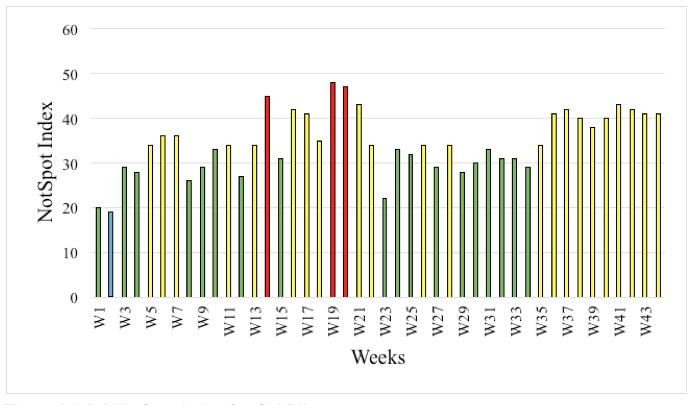
\includegraphics[width=1.0\linewidth]{notspot}
	\end{center}
	\vspace{-12pt}
	\caption{NotSpot Index for Citi Bike}
	\label{fig:heatmap}
\end{figure}

Once the current costs that systems incur for bike rebalancing have been determined, the incentives required to maintain system equilibrium may be examined. If these incentives represent a cost that is less than the current rebalancing costs, the intended approach is viable in that it will reduce operating expenditures for bike-share systems. Customer incentives currently play a role in the Paris and Cardiff systems. In Paris, riders are given an additional 15 minutes to return bikes to stations on hilltops, which are traditionally less popular return locations. In Cardiff, which is a relatively small system of approximately 150 bikes, riders are offered account credit that may be used to pay for overage fees for reverse riding, i.e. returning a bicycle back to the original location after the first leg of the trip is completed.

\subsection{Pricing Model}

In terms of pricing models, current systems rely on either subscription-based or pay-as-you-go models. However, research indicates that no prominent bike-share system incorporates a more dynamic pricing model. By determining the price of each ride in accordance to availability and user demand, it may be possible guarantee bike availability for users willing to pay, as well as indirectly reduce the rebalancing cost by incentivizing less common trips. This model, already used by many car-share systems and in a variety of other exchanges and markets, has the potential to increase profits and reduce costs by dynamically interacting with users. The approach involves studying existing dynamic pricing models, developing an algorithmic pricing model for bike-share systems, and testing it on existing data. \newline

Modeling decision-making is a challenge since numerous factors affect people's decisions, many of which are difficult to understand and quantify. Intangible factors affecting people's intrinsic motivations make it virtually impossible to come up with an algorithm representing an ``exact solution''. For example, despite efforts to account for environmental factors and geographic anomalies, some unknown social factor or local standard may cause unexpected behavior for an entire community. Furthermore, it has been shown that people's preferences are irrational and inconsistent--people often misjudge the worth of their time and spend a disproportional amount of time for a meager economic benefit, as long as the benefit is not framed as direct monetary compensation. Research will be conducted on studies of people's price elasticity in order to determine how to incentivize more balanced bike usage. Assumptions regarding human behavior and change in behavior as a result of monetary incentives will be included in the model. It will be assumed that customers will respond to monetary incentives, whether in the form of discounts, credit, or monetary rewards, and that they will exhibit price elasticity.\newline

Once a preliminary model is developed, simulations will be run using carefully selected dependent variables. Previous studies experienced problems regarding the multicollinearity of independent variables. To mitigate this concern, principal component analysis will be used.

\subsection{Mobile Application}
In conjunction with the algorithmic model for designing an effective bike-share, a smartphone application is being developed which will allow for real-world use of the system. The application indicates where bike stations are located, the availability of bikes at each nearby station, and the associated price for renting a bike for a specified time period, all updated in real-time based on live supply and demand. The application also provides the user with a list of trips the user may take to assist in rebalancing the system, rewarding users who partake in the effort with immediate monetary or credit rewards.\newline
Developing the application involves designing the user interface and coding the backend infrastructure. The app is currently being developed for iOS, and would be available to iPhone users. It is being developed in Swift using Xcode, and uses the GoogleMaps SDK, which provides a map interface on which nearby stations are presented to the user. The  Once the pricing algorithm has been refined, it will be incorporated into the logic so that the application can display availability and pricing schemes for users. \newline

A graphical representation of the entire system, including the available data, pricing model, bike station model, and software application, can be seen in Figure 2 below.


\begin{figure}[htb!]	\begin{center}
		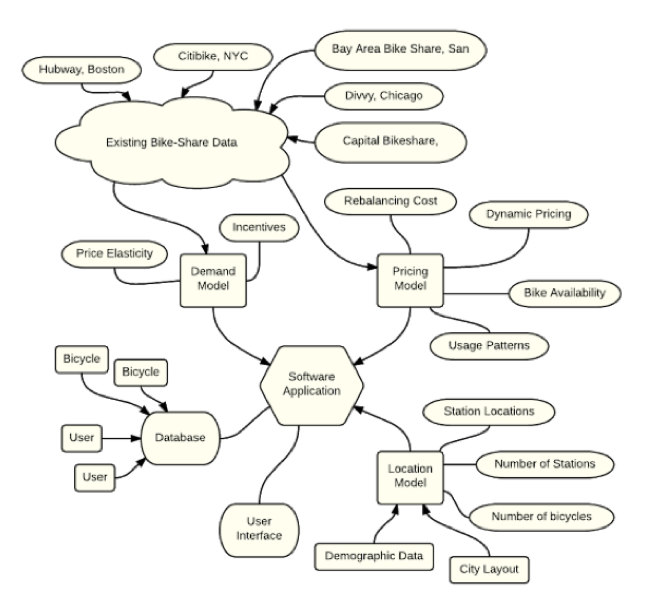
\includegraphics[width=1.0\linewidth]{model}
	\end{center}
	\vspace{-12pt}
	\caption{Model of Overall System}
	\label{fig:heatmap}
\end{figure}

\section{System Implementation}
\subsection{Rebalancing Approach}
Using existing historical data, we can create a 
\subsection{Pricing Model}
\subsection{Mobile Application}

\section{Remaining Work}

% We next move onto the bibliography.
\section{References}
\label{sec:references}
\begin{enumerate*}
\item "About Citi Bike." Citi Bike. N.p., 2014. Web. 28 Sept. 2014. <https://www.citibikenyc.com/about>. \newline

\item Buck, D. and R. Buehler. Bike Lanes and Other Determinants of Capital Bikeshare Trips. Presented at the 91st
Annual Meeting of the Transportation Research Board, Washington,  D.C., 2012. \newline

\item Daddio, D.W. Maximizing Bicycle Sharing: An Empirical Analysis of Capital Bikeshare Usage. University of North Carolina at Chapel Hill, 2012 \newline

\item Divvy. N.p., 2014. Web. 30 Sept. 2014. \newline<https://www.divvybikes.com/>. \newline

\item Gregerson, J., M. Hepp-Buchanan, D. Rowe, J. Vander Sluis, E. Wygonik, M. Xenakis, and E. McCormack. Seattle Bicycle Share Feasibility Study. University of Washington College of Built Environment Department of Urban Design and Planning, 2011. \newline

\item Gu, Jay. "Using Gradient Boosted Trees to Predict Bike Sharing Demand." GraphLab. N.p., 19 Aug. 2014. Web. 30 Sept. 2014. <http://blog.graphlab.com/using-gradient-boosted-trees-to-predict-bike-sharing-demand>. \newline

\item Johanson, Mark. "The World's Largest Bike-Share Programs." International Business Times. N.p., 30 May 2013. Web. 30 Sept. 2014. \newline<http://www.ibtimes.com/worlds-largest-bike-\newline share-programs-1283955>. \newline

\item Krykewycz, G.R., Puchalsky, C.M., Rocks, J., Bonnette, B., and F. Jaskiewicz. Defining a Primary Market Area and Estimating Demand for a Large-Scale Bicycle Sharing Program in  Philadelphia. In Transportation Research Record: Journal of the Transportation Research  Board, No. 2143, Transportation Research Board of the National Academies, Washington,  D.C., 2010, pp. 117-124 \newline

\item Maurer, L.K. Feasibility Study for a Bicycle Sharing Program in Sacramento, California. Presented at the 91st Annual Meeting of the Transportation Research Board, Washington, D.C., 2012.  \newline

\item Portland Business Alliance. "Re: Guiding Principles for Portland Bike Share Station Locations." (n.d.): n. pag. 15 Nov. 2012. Web. 30 Sept. 2014. \newline<http://portlandalliance.com/assets/111412-PDX-\newline Bike-Share-Guiding-Principles.pdf>. \newline

\item Press, Elizabeth. "The Biggest, Baddest Bike-Share in the World: Hangzhou China." Streetfilms. N.p., 1 June 2011. Web. 30 Sept. 2014. \newline<http://www.streetfilms.org/the-biggest-baddest-bike-share-in-the-world-hangzhou-china/>. \newline

\item Rixey, Alexander R. "Station-Level Forecasting of Bike Sharing Ridership : Station Network Effects in Three U.S. Systems." (n.d.): n. pag. 15 Nov. 2012. Web. 30 Sept. 2014. <http://docs.trb.org/prp/13-1862.pdf>. \newline

\end{enumerate*}
% Here is a dirty hack. We insert so much vertical space that the
% appendices, which want to begin in the left colunm underneath
% "references", are pushed over to the right-hand column. If we looked
% hard enough, there is probably a command to do exactly this (and
% wouldn't need tweaked after edits).
\vspace{295pt}

% We then use appendices to share some additional information with
% you, though you won't need appendices in your own proposal.
\appendix
\section{Figures}
\label{app:figures}

\end{document} 

